\subsection{示例 06：代码模板与工作区配置}

示例 \path{06_codegen_workspace} 为这一系列示例收尾。它展示的不是模型结构，而是所生成编辑器的行为。该领域包含一个根元素 \texttt{Program}、两个命令 \texttt{Log} 和 \texttt{Wait}，以及输出表达式 \texttt{BooleanLiteral}。此外，它还声明了语言 \texttt{javascript}、扩展名 \texttt{js}、执行类型 \texttt{workflow} 和 Blockly 工作区的可视化选项。适配器生成四种块类型、三个类别和四个等价模板；对比结果再次确认，双方生成的十个 HTML、JavaScript 和 JSON 产物完全相同。

\begin{figure}[H]
  \centering
  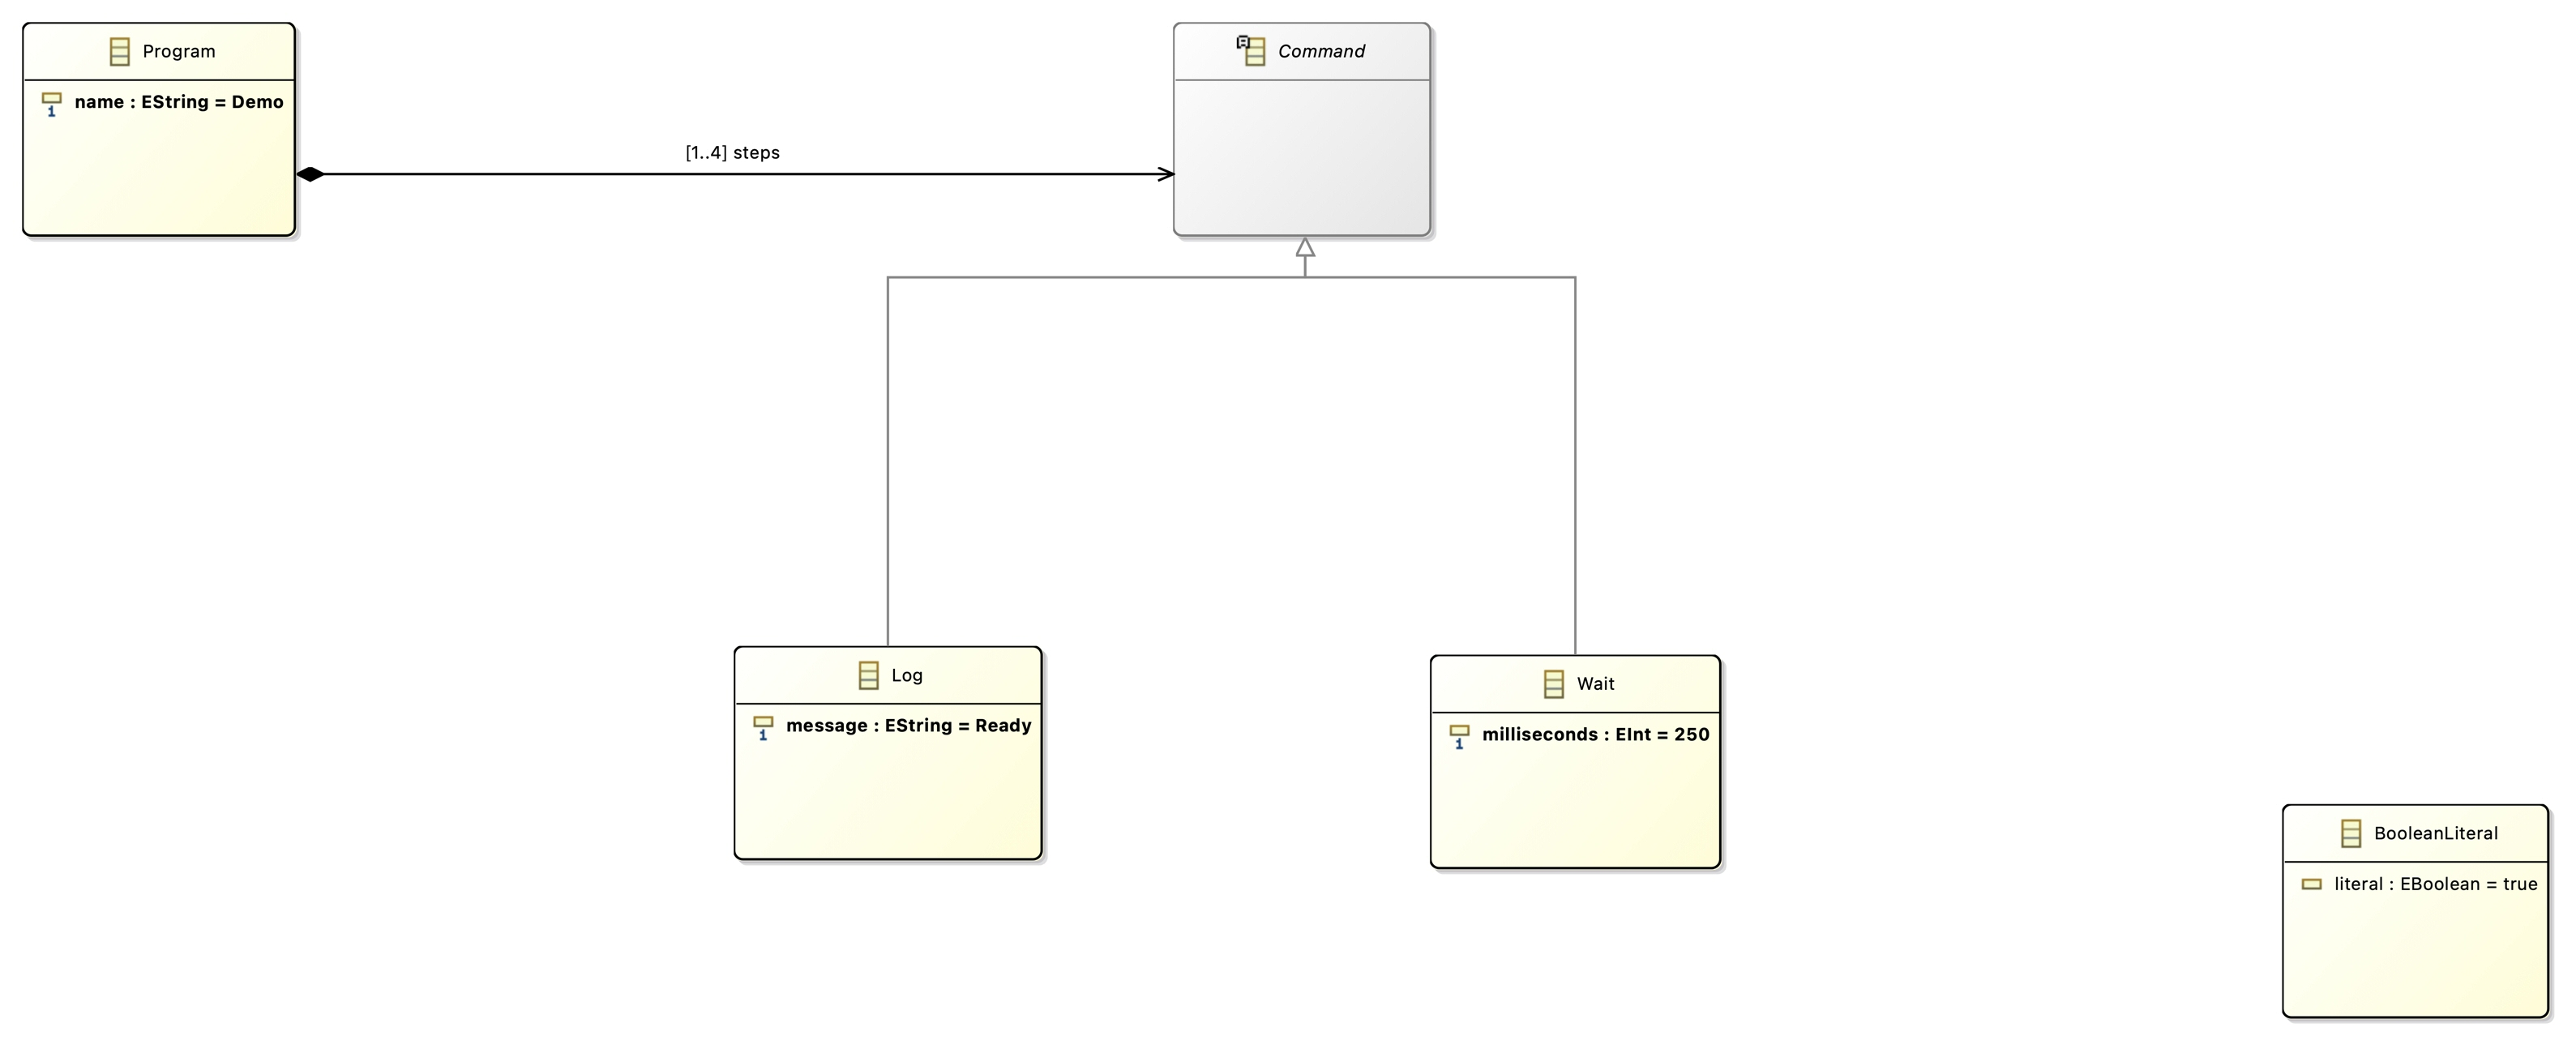
\includegraphics[width=\textwidth]{../../examples/feature_pairs/06_codegen_workspace/codegenWorkspace class diagram.jpg}
  \caption{示例 \texttt{06\_codegen\_workspace} 的 Ecore 类图}
  \label{fig:codegen-workspace-ecore}
\end{figure}

图 \ref{fig:codegen-workspace-ecore} 表明，\texttt{Program} 包含一个由一至四个 \texttt{Command} 元素组成的序列。\texttt{Command} 是抽象类，其具体子类 \texttt{Log} 和 \texttt{Wait} 分别提供一条消息和一个持续时间。\texttt{BooleanLiteral} 不属于该继承层次，因为它会转换为输出块，而不是序列中的命令。模型结构说明了哪些块可以连接；代码模板和工作区选项则保存在 Ecore 注解中，并在生成的编辑器里接受验证。

图 \ref{fig:codegen-workspace-editor} 展示了从 Ecore 得到的编辑器。文本路线的等价截图保存在 \path{screenshots/dsl.png}。左侧显示 \texttt{Program} 表单及其中包含的 \texttt{Log} 和 \texttt{Wait} 命令；右侧新增的 \emph{Code} 选项卡则显示根据同一工作区重新计算出的文本。因此，这项证据并非把编辑器与手工编写的输出进行比较，而是直接把已加载的块与模板生成结果对应起来。

\begin{figure}[H]
  \centering
  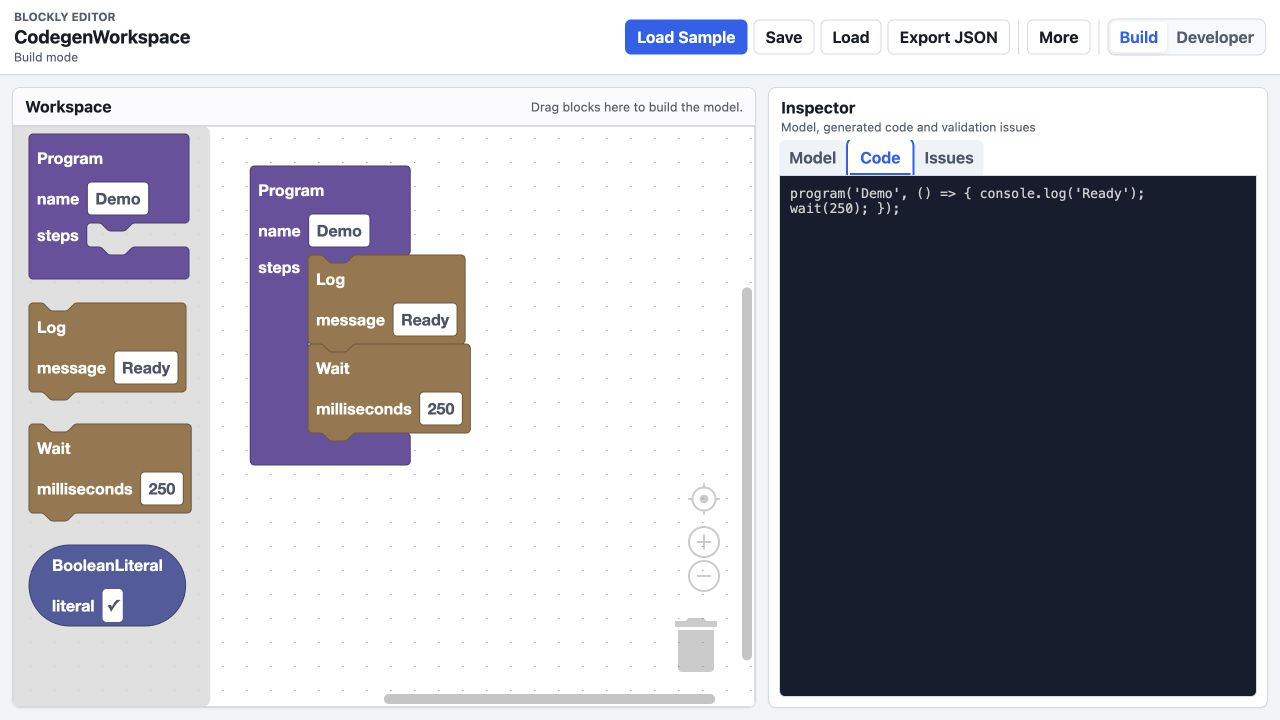
\includegraphics[width=\textwidth]{../../examples/feature_pairs/06_codegen_workspace/screenshots/ecore.png}
  \caption{加载示例模型并生成 JavaScript 代码后的
  \texttt{06\_codegen\_workspace} 编辑器}
  \label{fig:codegen-workspace-editor}
\end{figure}

可见文本调用了 \texttt{program}，参数包括名称 \texttt{Demo} 和一个先执行 \texttt{console.log}、再执行 \texttt{wait} 的函数。\texttt{Program} 的模板提供函数调用和函数体；\texttt{\{\{name\}\}} 被替换为 \texttt{Demo}；\texttt{\{\{statements:steps\}\}} 则遍历命令链。随后，每条命令应用自身的模板。包围 \texttt{Demo} 和 \texttt{Ready} 的引号来自模板：生成器只替换标记，不会尝试推断某种具体语言中的哪些值应当加引号。

表 \ref{tab:mapeo-codegen-workspace} 列出该示例集中展示的能力，并给出识别这些能力的证据。

\begin{table}[H]
  \centering
  \small
  \begin{tabular}{|L{0.27\textwidth}|L{0.28\textwidth}|L{0.31\textwidth}|}
    \hline
    输入 & 中间模型 & 可观察结果 \\
    \hline
    语言 \texttt{javascript} 和扩展名 \texttt{js} &
    \texttt{codeLanguage} 和 \texttt{codeFileExtension} &
    \emph{Code} 视图以及下载文件 \path{CodegenWorkspace_code.js}。 \\
    \hline
    \texttt{Program}、\texttt{Log} 和 \texttt{Wait} 的模板 &
    每个 \texttt{BlockTypeSpec} 的 \texttt{codeTemplate} &
    字段替换以及对 \texttt{steps} 的有序展开。 \\
    \hline
    声明为输出块的 \texttt{BooleanLiteral} &
    其 \texttt{BlockTypeSpec} 中的 \texttt{OUTPUT} 连接 &
    在工具箱中呈圆形，并可连接到值输入。 \\
    \hline
    执行类型 \texttt{workflow} &
    编辑器的 \texttt{runtimeKind} &
    可供执行环境及其控件使用的元数据。 \\
    \hline
    \texttt{renderer=zelos}、24 像素网格、吸附、缩放和垃圾桶 &
    类型化映射 \texttt{workspaceOptions} &
    在生成页面中配置好的网格、控件和渲染器。 \\
    \hline
    \texttt{flyout} 工具箱 &
    \texttt{toolboxType} 选项 &
    左侧常驻的块列表，不使用类别树。 \\
    \hline
  \end{tabular}
  \caption{\texttt{06\_codegen\_workspace} 中可观察到的转换}
  \label{tab:mapeo-codegen-workspace}
\end{table}

在 Ecore 路线中，\texttt{EcoreAdapter} 从包的 \texttt{code}、\texttt{runtime} 和 \texttt{blockly} 注解以及每个类的 \texttt{code} 注解获取这些数据。在文本路线中，\texttt{DomainModelAdapter} 读取领域属性、\texttt{workspace} 构造和每个类的 \texttt{code} 选项。两条路线都不会直接生成 JavaScript：它们首先填充 \texttt{EditorSpec} 中相同的字段。随后，\texttt{generateDomainCodegenBody} 为每种块类型输出一个配置映射，并生成在浏览器中解释模板的函数。

代码清单 \ref{lst:render-domain-statements} 展示了展开语句输入的部分。\texttt{block} 是所属块，在本例中为 \texttt{Program}；\texttt{inputName} 的值为 \texttt{steps}；\texttt{child} 指向当前处理的命令；\texttt{lines} 累积生成的文本；\texttt{rendered} 则包含应用某条命令模板后得到的结果。\texttt{getNextBlock} 调用保留了截图中可见的 \texttt{Log}--\texttt{Wait} 顺序。

\begin{lstlisting}[float=htbp, style=tfmjavascript, captionpos=t, caption={语句序列的模板展开过程}, label={lst:render-domain-statements}]
function renderDomainStatement(block, inputName) {
    var child = block.getInputTargetBlock(inputName);
    var lines = [];
    // 按 Blockly 连接顺序展开整条命令链。
    while (child) {
        var rendered = renderDomainBlock(child);
        if (rendered) lines.push(rendered);
        child = child.getNextBlock();
    }
    return lines.join('\n');
}
\end{lstlisting}

\texttt{applyDomainTemplate} 可识别三类标记：\texttt{\{\{name\}\}} 之类的简单字段、通过 \texttt{\{\{type\}\}} 表示的块类型，以及 \texttt{\{\{value:x\}\}} 或 \texttt{\{\{statements:x\}\}} 之类的结构输入。若缺少模板，\texttt{renderFallbackDomainBlock} 会保留通用文本表示，使导出功能在领域开发期间仍然可用。

\emph{Code} 选项卡在 \texttt{updateOutput} 中复用 \texttt{generateDomainCode(workspace)}；它使用 \texttt{textContent} 写入结果而不执行结果，并在每次变更后更新。\emph{Export Code} 选项调用同一函数，并使用 \texttt{codeFileExtension} 为下载文件命名。该示例的测试在两个页面中加载模型，检查四个模板、语言、扩展名和生成的 60 个字符，并在每个输出文件夹内将同一结果保存为 \path{html/sample_generated.js}。
\FloatBarrier

\subsection{Ecore 专用案例：元模型自身具备的能力}

Ecore 专用案例保存在目录：
\begin{center}
  \path{examples/ecore_specific/07_ecore_specific}
\end{center}
该案例检验 Ecore 原生具备而文本 DSL 尚无等价构造的信息，因此不纳入六个
双表示示例之间的等价性比较。

该元模型在根包中包含 \texttt{Catalog}，以 \texttt{NamedElement} 作为接口，并在子包 \texttt{details} 中包含 \texttt{Entry}。\texttt{Catalog} 包含抽象类型 \texttt{NamedElement} 的条目，并维护一个指向 \texttt{Entry} 的 \texttt{featured} 引用。具体类增加一个标识符和五个数值属性。此外，\texttt{Catalog} 还声明了四种技术属性——派生、瞬态、易失和不可修改——它们不应转换为可编辑控件。

\begin{figure}[H]
  \centering
  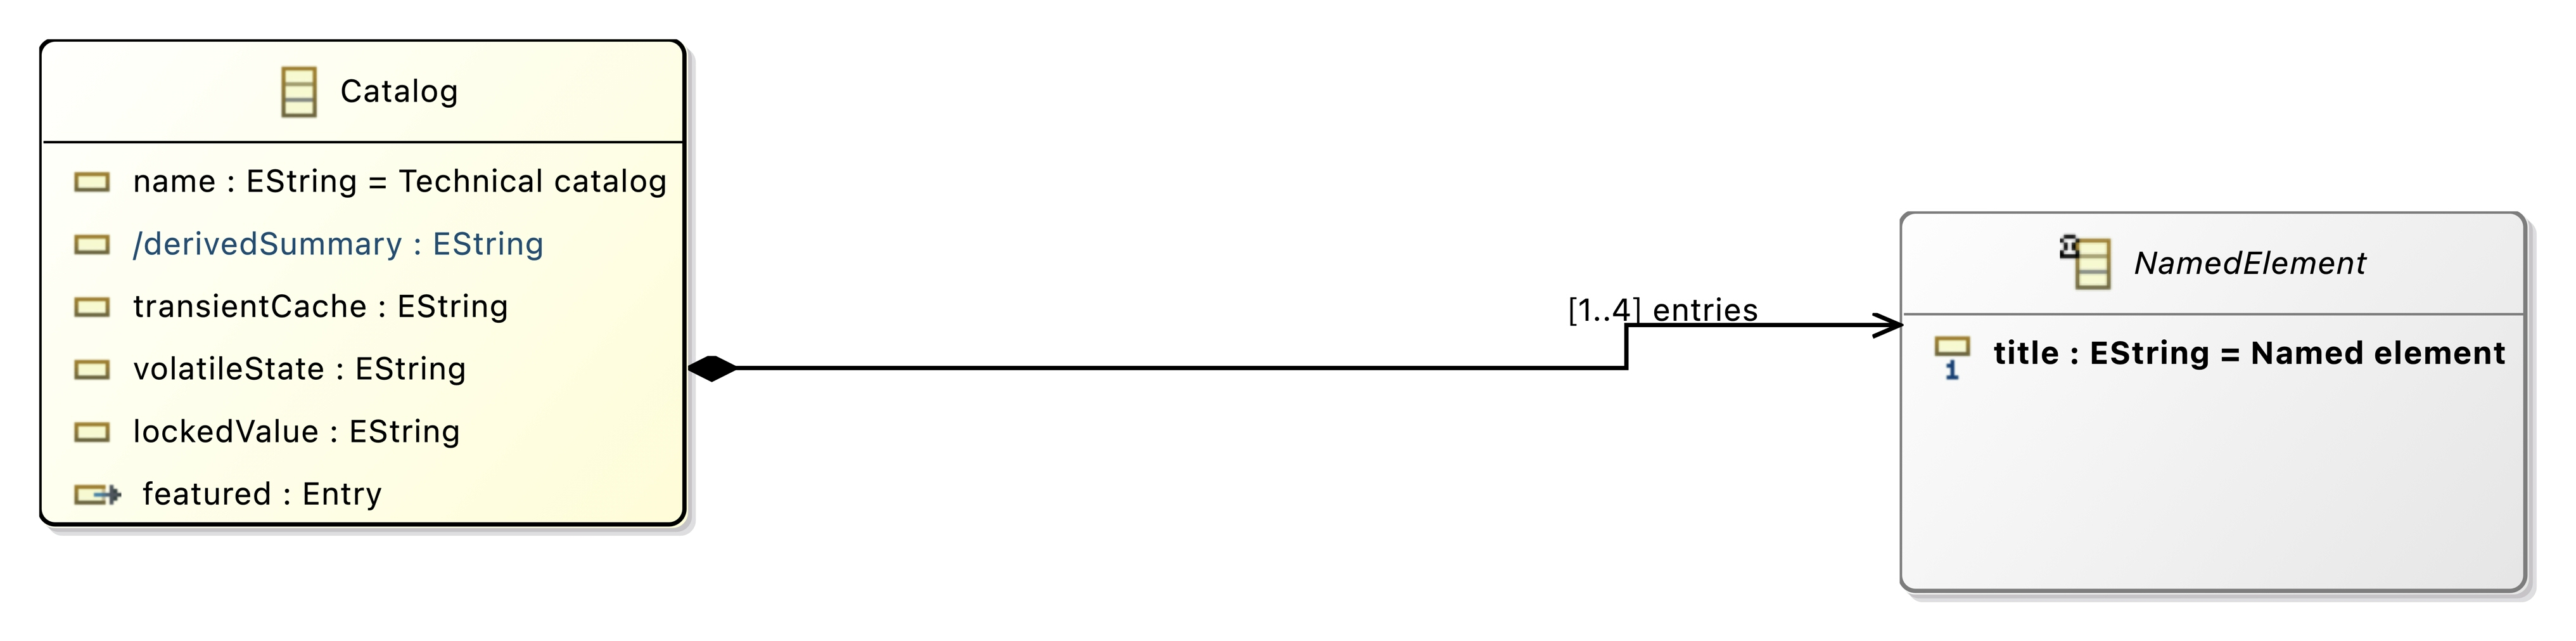
\includegraphics[width=\textwidth]{../../examples/ecore_specific/07_ecore_specific/ecoreSpecific class diagram.jpg}
  \caption{\texttt{07\_ecore\_specific} 案例的 Ecore 类图}
  \label{fig:ecore-specific-model}
\end{figure}

图 \ref{fig:ecore-specific-model} 展示了根包中的部分。\texttt{Catalog} 包含一至四个接口 \texttt{NamedElement} 类型的元素；位于子包 \texttt{details} 中的具体类型 \texttt{Entry} 是兼容实现，同时也是 \texttt{featured} 的目标。图中把 \texttt{derivedSummary} 标示为派生属性，并保留其余技术属性，以检验适配器会将它们过滤掉。必填属性 \texttt{title} 属于该接口，将由具体条目继承。

\begin{figure}[H]
  \centering
  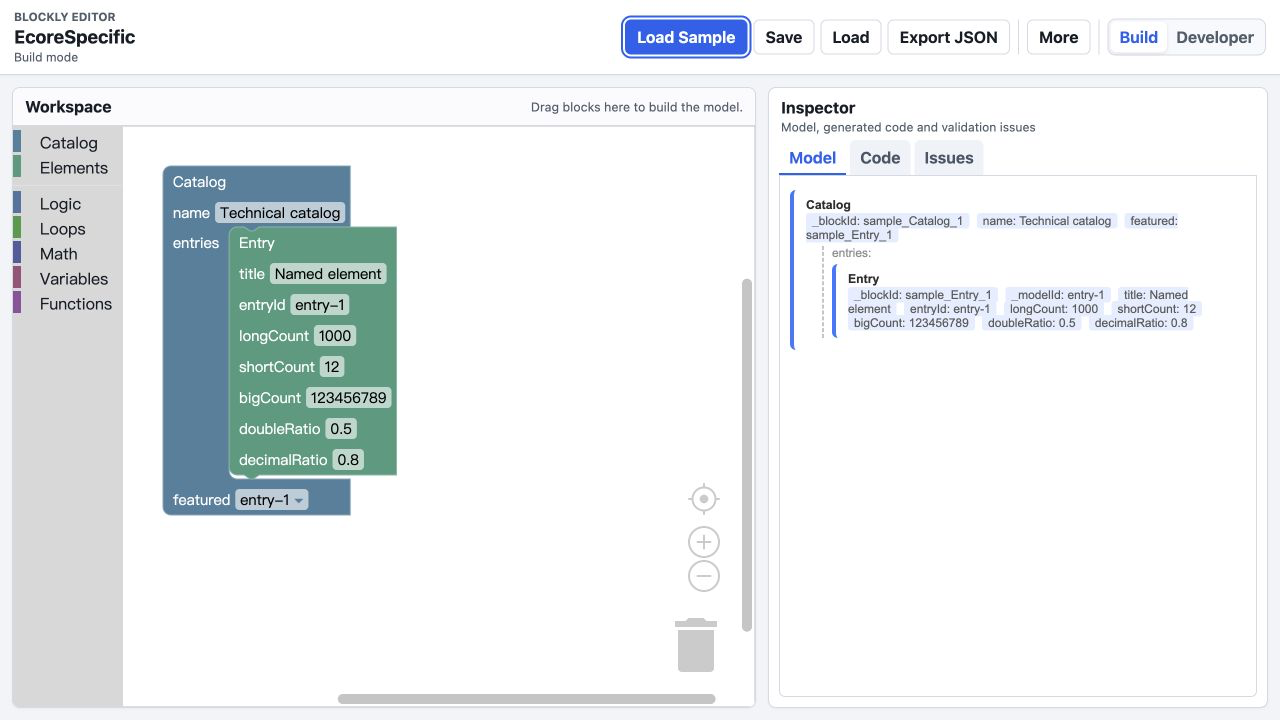
\includegraphics[width=\textwidth]{../../examples/ecore_specific/07_ecore_specific/screenshots/ecore.png}
  \caption{为 Ecore 专用能力生成的编辑器}
  \label{fig:ecore-specific-editor}
\end{figure}

蓝色的 \texttt{Catalog} 块只显示可编辑属性 \texttt{name}，被舍弃的四种技术属性均未出现。其 \texttt{entries} 输入能够接收绿色的 \texttt{Entry} 块，尽管该包含关系声明的是接口类型 \texttt{NamedElement}。在 \texttt{Entry} 中，\texttt{ELong}、\texttt{EShort} 和 \texttt{EBigInteger} 属性显示为整数，而 \texttt{EDouble} 和 \texttt{EBigDecimal} 显示为小数。最后，\texttt{featured} 下拉框使用 \texttt{entry-1}：适配器自动选择了被标记为标识符的 Ecore 属性 \texttt{entryId} 作为引用标签。检查器确认了生成模型中的相同值。

\begin{table}[H]
  \centering
  \scriptsize
  \begin{tabular}{|L{0.25\textwidth}|L{0.29\textwidth}|L{0.33\textwidth}|}
    \hline
    Ecore 能力 & 适配器中的实现 & 已核验的证据 \\
    \hline
    子包 \texttt{details} & 递归遍历
    \texttt{getESubpackages()} & 生成 \texttt{Entry}，且它可以从
    \texttt{Catalog} 连接。 \\
    \hline
    派生、瞬态、易失或不可修改的特征 &
    \texttt{isEditableFeature} 过滤器 & \texttt{Catalog} 的块和检查器
    只包含 \texttt{name}。 \\
    \hline
    \texttt{EClass.interface} & 接口转换为抽象块类型 &
    \texttt{NamedElement} 不会被实例化，但会作为 \texttt{entries}
    输入的类型。 \\
    \hline
    Ecore 数值别名 & 将 \texttt{ELong}、\texttt{EShort} 和
    \texttt{EBigInteger} 映射为 \texttt{INTEGER}，并将
    \texttt{EDouble} 和 \texttt{EBigDecimal} 映射为 \texttt{FLOAT} &
    \texttt{Entry} 中的五个字段均使用数值控件。 \\
    \hline
    自动引用标签 & 优先采用 ID 属性；随后尝试
    \texttt{displayName}、\texttt{title} 和 \texttt{name} &
    \texttt{featured} 显示 \texttt{entry-1}，即 \texttt{entryId} 的值。 \\
    \hline
    显式的 \texttt{nsURI} 和 \texttt{nsPrefix} & 复制到通用
    \texttt{EditorSpec} & 中间 XMI 保留源包中声明的这两个值。 \\
    \hline
    Ecore/OCL 注解 \texttt{HasTitle} & 转换为一条通用验证规则 &
    执行表达式包含 \texttt{has("title")}，并被纳入验证环境。 \\
    \hline
  \end{tabular}
  \caption{Ecore 专用能力的覆盖情况}
  \label{tab:ecore-specific-capabilities}
\end{table}

代码清单 \ref{lst:ecore-filter-subpackages} 展示可编辑特征过滤和子包递归遍历。
递归调用复用同一个分类器列表，确保 \texttt{details} 子包中的类型进入转换流程。

\begin{lstlisting}[style=tfmjavaecore, captionpos=t, caption={可编辑特征过滤与 Ecore 子包遍历}, label={lst:ecore-filter-subpackages}]
private static boolean isEditableFeature(EStructuralFeature feature) {
    return !feature.isDerived()
        && !feature.isTransient()
        && !feature.isVolatile()
        && feature.isChangeable();
}

private static List<EClassifier> allClassifiers(EPackage pkg) {
    List<EClassifier> result = new ArrayList<>();
    collectClassifiers(pkg, result);
    return result;
}

private static void collectClassifiers(EPackage pkg,
        List<EClassifier> result) {
    if (pkg == null) return;
    result.addAll(pkg.getEClassifiers());
    for (EPackage sub : pkg.getESubpackages()) {
        collectClassifiers(sub, result);
    }
}
\end{lstlisting}

其余能力由 \texttt{EcoreAdapter} 中的相应方法实现。当 \texttt{isAbstract()} 或 \texttt{isInterface()} 为真时，\texttt{convertEClass} 会把相应块标记为抽象块。属性转换按数值类型名称将其归入 \texttt{INTEGER} 和 \texttt{FLOAT} 两种统一类型。对于引用，\texttt{defaultReferenceLabelField} 首先尝试 \texttt{getEIDAttribute()}；仅在没有 ID 时，才应用约定名称。适配器还会复制 \texttt{nsURI} 和 \texttt{nsPrefix}，并把标准 OCL 注解转换到生成器使用的同一个验证模型中。

测试 \texttt{EcoreSpecificVerifierMain} 读取中间 XMI，并针对这七类能力进行断言。结果为 \texttt{7/7}；此外，浏览器测试会加载示例模型，并检查可见树、领域 XMI 和五条验证规则。因此，截图展示交互行为，而断言还验证了无法在单幅图像中直接观察的信息。
\FloatBarrier

\subsection{最终产物、HTML 封装页与导出}

最终生成阶段只接收经过规范化的 \texttt{EditorSpec}，并为两种输入路线生成
同一组文件；该阶段不再区分原始输入是 \texttt{.ecore} 还是 \texttt{.m2b}。

系统针对同一内容生成两个 HTML 封装页。\texttt{*\_editor.}\allowbreak\texttt{html} 页面分别加载块、工具箱、生成器和验证文件，便于嵌入页面并逐个调试模块。\texttt{*\_standalone.html} 页面则把领域专用 JavaScript 嵌入单个文档，以便演示。两种页面都从 \texttt{script} 标签指定的 CDN 加载 Blockly 库及其 JavaScript 生成器；因此，独立页面不包含 Blockly 的本地副本，打开时必须能够访问该依赖。

表 \ref{tab:artefactos-generados} 汇总了生成链路输出的主要文件。这份清单说明输出是可复现的完整结果，而不只是一个孤立的 HTML 页面。

\begin{table}[htbp]
  \centering
  \small
  \begin{tabular}{|L{0.32\textwidth}|L{0.54\textwidth}|}
    \hline
    生成的产物 & 内容 \\
    \hline
    \texttt{html/*\_blocks.js} & Blockly 块定义。 \\
    \texttt{html/*\_toolbox.js} & 编辑器的类别和工具箱。 \\
    \texttt{html/*\_generators.js} & 各个块的序列化函数和代码生成函数。 \\
    \texttt{html/*\_validations.js} & 在工作区上执行的验证规则。 \\
    \texttt{html/*\_editor.html} & 可嵌入的生成编辑器页面。 \\
    \texttt{html/*\_standalone.html} & 嵌入领域代码并从 CDN 加载 Blockly 的单页。 \\
    \texttt{html/sample\_model.json} & \texttt{Load Sample} 按钮使用的示例模型。 \\
    \path{html/validation_workspace.html} & 验证规则的可视化编辑器。 \\
    \path{html/validation_blocks.json} & 验证块的序列化树。 \\
    \path{html/validation_runtime.js} & 在浏览器中编译并评估可视化规则。 \\
    \path{intermediate/*_blocklyspec.xmi} & 生成 HTML 之前重新加载的 \texttt{EditorSpec} XMI 实例。 \\
    \texttt{generation\_report.html} & 生成过程的可追溯性报告。 \\
    \texttt{README.md} & 打开并检查结果的说明。 \\
    \hline
  \end{tabular}
  \caption{生成链路输出的主要产物}
  \label{tab:artefactos-generados}
\end{table}

在这些产物中，导出功能有两个目标。一方面，它把工作区序列化为 JSON 结构，其中包含块类型、标识符、字段、引用、值和语句。它还可以把这些内容导出为领域实例的 XMI，并使用输入包的前缀和 URI，避免把该 XMI 与中间 \texttt{EditorSpec} XMI 混淆。另一方面，系统还提供基于模板的代码生成路线。如果块定义了模板，生成器会用字段值、值输入或语句序列替换标记。如果没有模板，则使用通用文本表示。即使领域尚未定义完整的代码语义，这种策略仍可保持导出功能可用。

\section{运行时验证与引用}
\label{sec:implementacion-validaciones-referencias}

编辑过程中的引用同步和诊断由通用 JavaScript 运行时维持。实现区分两类验证：
一类是由 Eclipse/Xtext 在生成前完成的 DSL 静态验证；另一类是在浏览器中针对
Blockly 工作区执行的已构建模型验证。

\subsection{规则的编译与呈现}

\texttt{generateValidations}\allowbreak\texttt{Js} 生成函数 \texttt{computeValidation}\allowbreak\texttt{Warnings}、\texttt{applyValidation}\allowbreak\texttt{Warnings} 和 \texttt{init}\allowbreak\texttt{Validations}。第一个函数遍历 \texttt{workspace.}\allowbreak\texttt{getAllBlocks(false)}，并评估适用于每种类型的规则。如果活动的可视化模型中所有规则都有可转换的表达式，它会优先尝试执行该模型。如果不存在这个模型，或其中某条规则无法执行，则改用直接从 \texttt{EditorSpec} 输出的检查逻辑。顺序规则查询 \texttt{getPrevious}\allowbreak\texttt{Block}；基数规则沿着从 \texttt{getInputTarget}\allowbreak\texttt{Block} 开始的链进行检查；必填规则和唯一性规则则读取并比较字段值。\texttt{initValidations} 注册专用监听器，在创建、删除、移动或修改块之后重新执行计算。

规则也以树的形式保存在 \path{validation_blocks.json} 中。Java 类
\texttt{ValidationRuntime}\allowbreak\texttt{Generator} 把每棵树转换为执行环境所用的表达式，并生成 \path{validation_runtime.js}。在浏览器中，\texttt{createValidation}\allowbreak\texttt{Accessors} 提供 \texttt{value}、\texttt{has}、\texttt{inputCount}、\texttt{fieldUnique} 和 \texttt{previousBlockIs} 等受限操作；\texttt{evaluateRuntime}\allowbreak\texttt{Expression} 使用这些访问器执行表达式。借助这种表示方式，\path{validation_workspace.html} 可以显示编辑器实际使用的同一组规则，无需维护另一套独立的可视化定义。

代码清单 \ref{lst:apply-validation-warnings} 将同一块违反的多条规则按块标识符
合并，因为 Blockly 每个块只提供一段警告文本。

\begin{lstlisting}[style=tfmjavascript, caption={验证警告的合并与呈现}, label={lst:apply-validation-warnings}]
function applyValidationWarnings(workspace) {
    if (!workspace) return [];
    workspace.getAllBlocks(false).forEach(function(b) {
        b.setWarningText(null);
    });
    var warnings = computeValidationWarnings(workspace);
    var pending = {};
    warnings.forEach(function(w) {
        if (!w.block) return;
        if (!pending[w.block.id])
            pending[w.block.id] = { b: w.block, msgs: [] };
        pending[w.block.id].msgs.push(w.message);
    });
    Object.keys(pending).forEach(function(k) {
        var p = pending[k];
        p.b.setWarningText(p.msgs.join('\n'));
    });
    renderValidationIssues(warnings);
    return warnings;
}
\end{lstlisting}

\subsection{动态引用与相反引用}

非包含引用实现为以块标识符作为值的字段。生成的
\texttt{updateReference}\allowbreak\texttt{Dropdowns} 函数按类型对现有实例分组，为每个目标构建“标签--标识符”对，并替换下拉框选项。标签取自 \texttt{referenceLabel}\allowbreak\texttt{Field} 或 \texttt{name} 字段；若两者都没有，则最后使用类型和一部分标识符。如果被引用块被删除，其值将不再属于有效选项，因而会被清除。

此实现保持包含关系与引用之间的区别。包含关系在工作区中创建层次结构，而引用则选择已经存在的元素。这种分离方式保留了领域模型中的关系信息。

存在相反引用时，\texttt{synchronizeOppositeReferences} 会计算相反端的值并更新目标块。标志 \texttt{\_\_syncingOpposite}\allowbreak\texttt{References} 与暂时禁用事件的做法可以避免该写入操作引发通知循环。

\subsection{响应式协调与导出保护}

除了 \texttt{initValidations} 安装的专用监听器，引用脚本还会注册代码清单 \ref{lst:listener-runtime-blockly} 所示的协调监听器。\texttt{workspace} 仍表示当前 Blockly 工作区，\texttt{event} 描述一次变更：其 \texttt{type} 属性表示事件类别，\texttt{blockId} 标识块，\texttt{name} 则在适用时标识字段。通过 \texttt{typeof} 检查，即使某个领域不生成验证逻辑或输出视图，也能复用同一个监听器。

\begin{lstlisting}[style=tfmjavascript, caption={生成编辑器的响应式更新监听器}, label={lst:listener-runtime-blockly}]
workspace.addChangeListener(function(event) {
    if (event.type === Blockly.Events.BLOCK_MOVE ||
        event.type === Blockly.Events.BLOCK_CREATE ||
        event.type === Blockly.Events.BLOCK_DELETE ||
        event.type === Blockly.Events.BLOCK_CHANGE) {
        updateReferenceDropdowns(workspace);
        synchronizeOppositeReferences(workspace, event);
        if (typeof applyValidationWarnings === 'function')
            applyValidationWarnings(workspace);
        if (typeof updateOutput === 'function') updateOutput();
    }
});
\end{lstlisting}

在导出 JSON、XMI 或代码之前，\texttt{confirmExportIfInvalid} 会重新执行验证，并在仍有警告时请求确认。因此，用户可以检查不完整模型而不会阻塞编辑，但导出过程不会掩盖其中的问题。数值边界 \texttt{min} 和 \texttt{max} 会直接写入 Blockly 字段。

\subsection{检查、可视化编辑与环境限制}

页面还包含一个通用模型检查执行器。

\texttt{generateRuntimeScript} 方法根据模型生成相应代码。在执行期间，该代码把工作区转换为领域的 JSON 表示，递归遍历其中的节点，并通过运行、暂停和单步控件高亮当前访问的块。它不执行各个领域的具体语义；其作用是观察已构建的结构，并检查模型的遍历顺序。

补丁工具补全了验证闭环。可以从命令行对 \texttt{validation\_blocks.edited.json} 文件运行该工具，也可以通过 Eclipse 中的 \texttt{Apply Validation Blocks to Source} 调用。补丁采用保守策略：只更新能够明确映射到文本语法或 Ecore 注解的规则，不处理无法直接转换的表达式。

生成的运行时机制有意保持轻量化。它既不是完整的 OCL 引擎，也不是通用语义验证器。其覆盖范围包括基数、必填性、唯一性、相反引用、已声明表达式，以及适配器能够转换为 JavaScript 可用访问器的 OCL 不变量子集。

\section{Eclipse 集成与分发}
\label{sec:implementacion-eclipse-distribucion}

\subsection{命令注册与处理器执行}

Eclipse 集成声明在界面 bundle 的 \texttt{plugin.xml} 文件中。该文件注册
\texttt{generateBlockly}\allowbreak\texttt{Editor} 和
\texttt{applyValidation}\allowbreak\texttt{Patch} 命令，将它们分别关联到
\texttt{GenerateBlockly}\allowbreak\texttt{EditorHandler} 和
\texttt{ApplyValidation}\allowbreak\texttt{PatchHandler}，并仅在选中一个兼容文件时显示这些命令。上下文菜单项支持 \texttt{.ecore} 和 \texttt{.m2b}；同时保留历史扩展名 \texttt{.model2blockly}，以便打开旧项目。

\texttt{GenerateBlockly}\allowbreak\texttt{EditorHandler} 扩展
\texttt{AbstractHandler}。其 \texttt{execute} 方法获取所选的 \texttt{IFile}，检查扩展名，并把工作委托给由 Eclipse 进度服务执行的
\texttt{IRunnableWith}\allowbreak\texttt{Progress}。这种委托可以避免在加载 EMF 资源、生成中间 XMI 和创建 Web 产物期间阻塞界面。

代码清单 \ref{lst:eclipse-generate-runnable} 展示 runnable 的核心。条件表达式
选择 Ecore 或文本加载路线，两个分支均返回“相对路径--文本内容”映射并汇合到
\texttt{writeFiles}；异常被包装为
\texttt{InvocationTarget}\allowbreak\texttt{Exception} 后返回处理器。

\begin{lstlisting}[style=tfmjava, caption={Eclipse 生成路线的选择与执行}, label={lst:eclipse-generate-runnable}]
@Override
public void run(IProgressMonitor monitor)
        throws InvocationTargetException {
    try {
        monitor.beginTask("Generating Blockly editor",
            IProgressMonitor.UNKNOWN);
        Map<String, String> files =
            "ecore".equals(inputFile.getFileExtension())
                ? generateFromEcore(inputFile)
                : generateFromModel2Blockly(inputFile);
        writeFiles(inputFile, files, monitor);
    } catch (Exception e) {
        throw new InvocationTargetException(e);
    } finally {
        monitor.done();
    }
}
\end{lstlisting}

两个分支都复用第 \ref{sec:carga-validacion-entradas} 节的加载逻辑、第 \ref{sec:implementacion-ecore-adapter} 节和第 \ref{sec:implementacion-domainmodel-adapter} 节的适配器，以及第 \ref{sec:implementacion-generador-html} 节的生成器。两种情况下都会在序列化 \texttt{EditorSpec} 之前验证它，重新加载其 XMI，并在生成 HTML 和 JavaScript 之前进行第二次验证。

\subsection{在工作区中写入产物}

两个分支的共同结果是传递给 \texttt{writeFiles} 的产物映射。该方法计算 \texttt{*\_generated} 文件夹，递归创建其子目录，并删除已知的过时输出。对于映射中的每个条目，它获取一个 \texttt{IFile}，将内容转换为 UTF-8；若资源不存在，则使用 \texttt{IFile.create}，需要更新时则使用 \texttt{IFile.setContents}。完成后，它刷新项目，在 \emph{Project Explorer} 中显示文件夹，并在 workbench 中打开 \texttt{generation\_report.html}。

\subsection{诊断与验证回写}

该集成还会将转换故障接入 IDE 的诊断机制。如果 \texttt{EditorSpec} 验证失败，\texttt{BlocklySpecSourceMapper} 可以在源元素上创建 \texttt{IMarker.PROBLEM}，并在信息可用时包含行号、位置、消息和建议。Xtext 生成的错误也会以同样方式转换为与 \texttt{.m2b} 文件关联的标记。因此，用户收到的不只是一个 Java 异常：源编辑器会打开，Eclipse 还会显示问题位置。

\texttt{ApplyValidation}\allowbreak\texttt{PatchHandler} 为可视化编辑后的规则实现反向流程。处理器会推荐对应输出中的 \path{validation_blocks.json} 文件，首先执行
\texttt{ValidationPatch}\allowbreak\texttt{Service.dryRun}，并在请求确认前展示变更。只有在确认后，它才执行 \texttt{apply}、刷新资源并重新打开源文件。当写入目标与源文件相同时，服务会预先保留一个扩展名为 \texttt{.bak} 的副本。因此，在用户查看 \emph{dry-run} 摘要并确认所提议的变更之前，回写流程不会修改源文件。

\subsection{p2 打包与交付产物}

可安装分发包分两个层级实现。\texttt{feature.xml} 文件把主 bundle、IDE bundle 和 UI bundle 归入 feature \path{io.github.plortinus.model2blockly.feature}。随后，\texttt{category.xml} 在 p2 仓库的 Model2Blockly 类别中发布该 feature。此仓库包含三个 bundle 的 JAR，以及元数据 \texttt{content.jar} 和 \texttt{artifacts.jar}；这样，无需导入源项目，即可通过 \texttt{Help -> Install New Software} 安装本章所述的同一实现。

仓库还会发布源代码、p2 仓库、六个双表示示例、Ecore 专用案例及其生成输出。对于每个示例，\path{generated/ecore} 和 \path{generated/dsl} 目录都包含报告、中间 XMI、示例模型、验证规则和编辑器。因此，无需再次执行转换即可检查两条路线。表 \ref{tab:artefactos-entrega} 汇总了交付所用的访问入口。

\begin{table}[htbp]
  \centering
  \small
  \begin{tabular}{|L{0.24\textwidth}|L{0.62\textwidth}|}
    \hline
    产物 & 位置 \\
    \hline
    源代码 &
    \url{https://github.com/Plortinus/model2blockly} \\
    p2 仓库 &
    \url{https://plortinus.github.io/model2blockly/update-site/} \\
    项目网站 &
    \url{https://plortinus.github.io/model2blockly/} \\
    Ecore 与 \texttt{.m2b} 双表示示例 &
    \url{https://github.com/Plortinus/model2blockly/tree/main/examples/feature_pairs} \\
    评估语料库 &
    \url{https://github.com/Plortinus/model2blockly/tree/main/evaluation/official-blockly} \\
    交付文档 &
    \path{README.md}、\path{DOCS.md} 和
    \path{examples/feature_pairs/README.md} \\
    \hline
  \end{tabular}
  \caption{Model2Blockly 仓库的交付产物}
  \label{tab:artefactos-entrega}
\end{table}
\FloatBarrier

\section{独立入口}
\label{sec:implementacion-standalone}

\subsection{可用接口与两个入口的汇合}

主 bundle 提供三个无需 workbench 即可执行的 Java 入口，代码清单 \ref{lst:entradas-standalone} 对其进行了汇总。

\begin{lstlisting}[style=tfmcli, caption={独立入口的命令行接口}, label={lst:entradas-standalone}]
// 从 Ecore 文件加载的 EPackage 生成。
EcoreToBlocklyMain <file.ecore> [output-dir]
// 从 Xtext 解析出的 DomainModel 生成。
Model2BlocklyToBlocklyMain <file.m2b> [output-dir]
// 对源文件应用或模拟验证变更。
ValidationPatchMain --source <file> --validation <json> [options]
\end{lstlisting}

\texttt{EcoreToBlocklyMain} 是 Ecore 路线的入口。它注册资源工厂，加载 \texttt{EPackage} 并执行 \texttt{EcoreAdapter}。随后，它验证并重新加载中间 XMI，再把结果传递给 \texttt{BlocklyCodeGenerator}。

\texttt{Model2BlocklyToBlocklyMain} 实现文本路线。它使用 Xtext 生成的独立配置创建 Guice 注入器，获取 \texttt{XtextResource}，执行语法和语义验证，并调用 \texttt{DomainModelAdapter}。从 \texttt{EditorSpec} 开始，两个类完全复用同一套最终生成逻辑。历史扩展名 \texttt{.model2blockly} 与 \texttt{.m2b} 使用同一分支，不存在第三个适配器。

\subsection{输出路径解析与磁盘写入}

如果省略第二个参数，两个入口都会删除源文件扩展名，并在源文件所在位置创建
\texttt{<name>}\allowbreak\texttt{\_generated} 目录；没有父目录时使用当前工作目录。

\begin{lstlisting}[style=tfmjava, caption={独立入口的默认输出目录计算}, label={lst:standalone-default-output}]
private static String defaultOutputDir(String inputPath) {
    File input = new File(inputPath);
    String name = input.getName();
    int dot = name.lastIndexOf('.');
    if (dot > 0)
        name = name.substring(0, dot);
    File parent = input.getParentFile();
    return new File(parent != null ? parent : new File("."),
        name + "_generated").getPath();
}
\end{lstlisting}

Blockly 产物写入 \texttt{html/} 下；中间 XMI、README 和报告则写入与插件相同的目录结构。映射中的每个条目都会转换为 \texttt{File}；系统创建其父目录，并由 \texttt{FileWriter} 写入内容。控制台为每个生成文件输出一行，并在结束时显示报告、编辑器、中间模型和验证工作区的绝对路径。表 \ref{tab:standalone-exit-codes} 明确说明了两个生成器所采用的退出约定。

\begin{table}[H]
  \centering
  \small
  \begin{tabular}{|>{\centering\arraybackslash}p{0.12\textwidth}|L{0.68\textwidth}|}
    \hline
    代码 & 含义 \\
    \hline
    0 & 生成成功，或查询 \texttt{--help}。 \\
    1 & 缺少必填参数，或位置参数过多。 \\
    2 & 未知选项，或目标不是 HTML。 \\
    3 & 加载、解析、适配或验证失败。 \\
    4 & 至少一个产物无法写入磁盘。 \\
    \hline
  \end{tabular}
  \caption{独立生成器的退出代码}
  \label{tab:standalone-exit-codes}
\end{table}

对退出代码进行区分，便于把可执行程序集成到构建脚本中：源文件故障与输出写入问题可以明确区分。

\subsection{从命令行回写验证规则}

\texttt{ValidationPatchMain} 复用 \texttt{ValidationSourcePatcher} 来执行验证回写流程。默认模式为 \texttt{--dry-run}；\texttt{--apply} 会写入变更，\texttt{--out} 则可以保持原始源文件不变。第三个入口还用于自动检查应用补丁后的模型能否重新生成编辑器。内部类 \texttt{Options} 保存 \texttt{source}（将被修改的源文件）、\texttt{validation}（编辑后的 JSON）、\texttt{output}（可选输出）以及布尔值 \texttt{apply}。解析参数后，最后这个值用于选择 \texttt{ValidationSourcePatcher.apply} 或 \texttt{ValidationSourcePatcher.dryRun}；生成的 \texttt{PatchReport} 会把变更、警告和说明输出到控制台。
\FloatBarrier

\section{实现测试}
\label{sec:implementacion-pruebas}

\subsection{按组件划分的单元测试}

该实现包含 145 个 JUnit~5 测试方法。统计范围是 \texttt{test} 目录中的六个类，其分布如表 \ref{tab:pruebas-implementacion} 所示。

\begin{table}[htbp]
  \centering
  \small
  \begin{tabular}{|L{0.62\textwidth}|>{\centering\arraybackslash}p{0.18\textwidth}|}
    \hline
    测试类 & \texttt{@Test} 方法数 \\
    \hline
    \texttt{BlocklyCodeGeneratorTest} & 61 \\
    \texttt{BlocklyEditorSpecTest} & 27 \\
    \texttt{DomainModelAdapterTest} & 8 \\
    \texttt{EcoreAdapterTest} & 39 \\
    \texttt{GeneratedBlocklySpecModelTest} & 5 \\
    \texttt{Model2BlocklyValidatorBridgeTest} & 5 \\
    \hline
    合计 & 145 \\
    \hline
  \end{tabular}
  \caption{实现层 JUnit 测试方法分布}
  \label{tab:pruebas-implementacion}
\end{table}

中间模型测试检查默认值、字段类型、连接、抽象块过滤和 XMI 序列化。适配器测试针对两条路线检查类、属性、引用、继承、基数、注解和代码元数据。规模最大的一组是生成器测试：它检查产物名称、HTML 结构、块、工具箱、验证、引用、工作区持久化，以及 JSON、XMI 和代码导出。验证桥接类通过独立配置创建 Xtext 资源，并验证 DSL 诊断会在适配前传播。

\subsection{集成验证与浏览器验证}

\texttt{package.json} 文件声明了结合 Java 类、Node.js 脚本、EMF 和真实浏览器的验证任务。表 \ref{tab:implementation-verification-commands} 说明了每个命令检查的约定；这些命令并非重复同一项度量，而是覆盖互补层级，并定位不同类型的故障。

\begin{table}[H]
  \centering
  \small
  \begin{tabular}{|L{0.27\textwidth}|L{0.58\textwidth}|}
    \hline
    命令 & 检查的约定 \\
    \hline
    \texttt{verify:plugin} & 清单、\texttt{plugin.xml}、feature、JAR、p2 仓库以及分发包所含示例之间的一致性。 \\
    \hline
    \texttt{verify:patch} & 模拟、应用验证回写并检查其幂等性，随后重新执行 Ecore 生成。 \\
    \hline
    \texttt{verify:domain-xmi} & 使用 EMF 加载生成编辑器所导出的实例 XMI。 \\
    \hline
    \texttt{verify:docs} & 英文、西班牙文和中文文档版本中的路径及必备页面是否对应。 \\
    \hline
    \texttt{smoke} & 打开每个指定编辑器，加载示例模型，并检查 Blockly 工作区、检查器、验证及可观察的导出结果。 \\
    \hline
    \texttt{verify:feature-pairs} & 生成六个双表示示例，对 \texttt{EditorSpec} 进行规范化比较，执行能力断言，并对十二个编辑器和 Ecore 专用案例运行 \texttt{smoke}。 \\
    \hline
  \end{tabular}
  \caption{实现的自动化验证}
  \label{tab:implementation-verification-commands}
\end{table}

在最近一次执行中，六个双表示示例均通过生成与对比；Ecore 示例通过七组断言；十三个编辑器均通过浏览器测试。由此，Java 约定、两条路线的等价性、没有文本等价构造的能力、Eclipse 打包以及生成 HTML 的实际行为都得到了分别验证。

\subsection{与评估的区分}

这些测试回答的是实现是否满足既定契约：有效输入能否在不丢失信息的情况下完成转换，产物能否打开，以及生成的函数能否按预期响应。它们本身不能证明 Model2Blockly 降低了重建现有编辑器所需的工作量，也不能证明其结果等价于官方参考实现。这些问题需要外部案例、度量和验收标准；因此留到第~\ref{chap:evaluacion}章讨论。

\section{实现总结}
\label{sec:resumen-implementacion}

Model2Blockly 的实现允许通过带注解的 Ecore 或文本路线 \texttt{.m2b} 定义领域。两个入口都会转换为同一个 \texttt{EditorSpec}，在 XMI 序列化前后接受验证，并复用 HTML/JavaScript 生成器。基于这一约定，系统生成块、工具箱、验证、动态引用、导出器、报告、可视化验证工作区和代码模板。

同一生成链还通过 Eclipse 命令和独立 Java 入口提供。feature 和 p2 仓库负责分发插件；JUnit 测试、打包测试和浏览器冒烟测试则覆盖互补层级。因此，该实现以中间模型为核心，具体落实了上一章定义的生成式架构。
